\documentclass[t]{beamer}
\usefonttheme[onlymath]{serif}

\mode<presentation>
{
  \usetheme{Frankfurt}
  \usecolortheme{dove}  %% grey scale
  \useinnertheme{circles}
  % \setbeamercovered{transparent}
}

\hypersetup{
    colorlinks,
    citecolor=black,
    filecolor=black,
    linkcolor=black,
    urlcolor=blue
}
\usepackage{graphicx}

\graphicspath{ {../folding/sonobe-docs/src/imgs} }

\usepackage{listings} % embed code

\setbeamertemplate{itemize}{$\circ$}
\setbeamertemplate{itemize items}{$\circ$}

\beamertemplatenavigationsymbolsempty %% no navigation bar

\setbeamertemplate{footline}{\hspace*{.1cm}\scriptsize{
\hspace*{50pt} \hfill\insertframenumber/\inserttotalframenumber\hspace*{.1cm}\vspace*{.1cm}}}

\setbeamertemplate{caption}[numbered]
\setbeamerfont{caption}{size=\tiny}


\title{An overview on folding schemes,\\and an introduction to Sonobe}
\author{
  % Folding polynomials and proving it onchain.\\
  % \small{Sonobe: experimental folding schemes library implemented jointly by \href{https://0xparc.org}{0xPARC} and \href{https://pse.dev/}{PSE.}}\\
  \vspace{0.2cm}
  
\includegraphics[width=3cm]{sonobe}
}

\date{\vspace{0.1cm}\scriptsize{2024-08-08\\San Francisco 0xPARC Summer}}

\begin{document}

\frame{\titlepage}



\section[Motivation]{Motivation}

\begin{frame}{Polynomials and SNARKs}
  \begin{itemize}
    \item define the 'program' that we want to be able to prove as a set of constraints
    \item encode the constraints as polynomials
    \\eg. R1CS: $Az \circ Bz - Cz == 0$
    \\~~~~~~~~~~$A(X) \cdot B(X) - C(X) == 0$
    \item and then use some scheme to prove that those polynomials satisfy the relation. eg. Groth16, Spartan, etc
  \end{itemize}
  tl;dr: want to prove polynomial relations
\end{frame}

\begin{frame}{Why folding}
  \begin{itemize}
    \item Repetitive computations take big circuits $\longrightarrow$ large proving time
    \begin{itemize}
      \item and in some cases takes too much memory and can not be even computed
      \item eg. prove a chain of 10k sha256 hashes (>600M R1CS constraints, not feasible with most traditional SNARK proving systems)
    \end{itemize}

    % \pause

    \item Traditional recursion: verify (in-circuit) a proof of the correct execution of the same circuit for the previous input
    \begin{itemize}
      \item issue: in-circuit proof verification is expensive (constraints)
      \begin{itemize}
        \item ie. verify a Groth16 proof inside a R1CS circuit
      \end{itemize}
    \end{itemize}
  \end{itemize}

  % DRAW: G16 proof being verified inside a circuit for which a new proof is generated
\end{frame}

\begin{frame}{IVC - Incremental Verifiable Computation}
  {\tiny Valiant'08}\\
  Folding schemes efficitently achieve IVC, where the prover recursively proves the correct execution of the incremental computations.
  \vspace{0.5cm}

  % For a function $F$, with initial input $z_0$, an IVC scheme allows a prover to produce a proof $\pi_i$ for the statement $z_i=F^{(i)}(z_0)$, given a proof $\pi_{i-1}$ for the statementkj
  \emph{Prove that applying $n$ times the $F$ function (the circuit being folded) to the initial state ($z_0$) results in the final state ($z_n$).}


  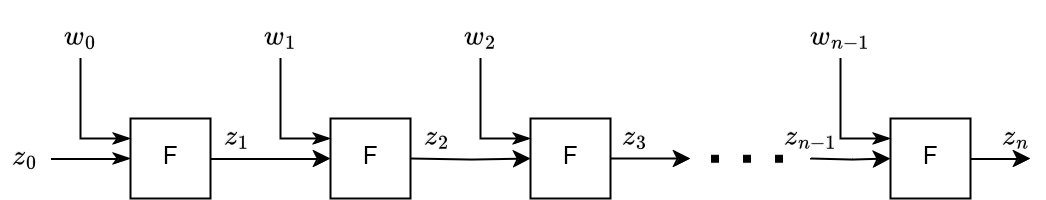
\includegraphics[width=\textwidth]{folding-main-idea-diagram}

  In other words, it allows to prove efficiently that $z_n = F(...~F(F(F(F(z_0, w_0), w_1), w_2), ...), w_{n-1})$.
\end{frame}


\begin{frame}{Folding idea}
  % DRAW of 2 instances being folded into a single one
  % then add other instances to show k-to-1 folding
\end{frame}


% \section[Folding]{Folding}
% \begin{frame}{Fold polynomials - a simple example}
%   TODO example folding poly
% \end{frame}

\begin{frame}{Random linear combination of homomorphic commitments}
  \small{
    We rely on homomorphic commitments, eg. Pedersen commitments\\
  }

  Let $g \in \mathbb{G}^n,~ v \in \mathbb{F}_r^n$,\\
  $$Com(v) = \langle g, v \rangle =g_1 \cdot v_1 + g_2 \cdot v_2 + \ldots + g_n \cdot v_n \in \mathbb{G}$$

  RLC:\\
  Let $v, w \in \mathbb{F}_r^n$,
  \\set $cm_v = Com(v),~ cm_w=Com(w) \in \mathbb{G}$.
  \\then,
  \begin{align*}
    y &= v + r \cdot w\\
    cm_{y} &=cm_v + r \cdot cm_w
  \end{align*}
  \\so that
  $$cm_y = Com(y)$$

\end{frame}

\begin{frame}{Relaxed R1CS}
  % TODO: think if maybe remove this slide and the next one (NIFS)\\

  R1CS instance: $(\{A, B, C\} \in \mathbb{F}^{n \times n},~ n,~ l)$, such that for $z=(1, io \in \mathbb{F}^l, w \in \mathbb{F}^{n-l-1}) \in \mathbb{F}^n$,

$$Az \circ Bz = Cz$$

% \pause

Relaxed R1CS:

$$Az \circ Bz = uCz + E$$

for $u \in \mathbb{F},~~ E \in \mathbb{F}^n$.

\vspace{1cm}

Committed Relaxed R1CS instance: $CI = (\overline{E}, u, \overline{W}, x)$\\
Witness of the instance: $WI=(E, W)$

\end{frame}

\begin{frame}{Relaxed R1CS}
  % \vspace{-1cm}
  \scriptsize{
	$u=u_1+r u_2,~~ z=z_1+r z_2,~~ x=x_1+r x_2$\\
	$E=E_1 + r (A z_1 \circ B z_2 + A z_2 \circ B z_1 - u_1 C z_2 - u_2 C z_1) + r^2 E_2$\\
  \text{Relaxed R1CS:} $Az \circ Bz = uCz + E,~~ with~ z=(u,~x,~W)$
\begin{align*}
	Az \circ Bz 
            &= A(z_1 + r \cdot z_2) \circ B(z_1 + r \cdot z_2)\\
            &= A z_1 \circ B z_1 + r(A z_1 \circ B z_2 + A z_2 \circ B z_1) + r^2 (A z_2 \circ B z_2)\\
            &= (u_1 C z_1 + E_1) + r (A z_1 \circ B z_2 + A z_2 \circ B z_1) + r^2 (u_2 C z_2 + E_2)\\
            &= u_1 C z_1 + \underbrace{E_1 + r(A z_1 \circ B z_2 + A z_2 \circ B z_1) + r^2 E_2}_\text{E} + r^2 u_2 C z_2\\
            &= u_1 C z_1 + r^2 u_2 C z_2 + E\\
            &= (u_1 + r u_2) \cdot C \cdot (z_1 + r z_2) + E\\
            &= uCz + E
\end{align*}

For R1CS matrices $(A,~B,~C)$, the folded witness $W$ is a satisfying witness for the folded instance $(E,~u,~x)$, following the Relaxed R1CS relation: $Az \circ Bz - uCz - E ==0$.

Since we don't want that the Verifier learning about the witness, we commit to it, and the Verifier will run the RLC on the commitment (not on the witness), obtaining the 'folded' commitment.

\\\tiny{Full details at Nova's paper, pages 13-15 ("first attempt, second attempt, third attempt")}
}
\end{frame}
% \begin{frame}{NIFS - Non Interactive Folding Scheme (in Nova)}
%   \vspace{-0.5cm}
%   \scriptsize{
%   \begin{align*}
%     CI_1 &=(\overline{E}_1 \in \mathbb{G}, u_1 \in \mathbb{F}, \overline{W}_1 \in \mathbb{G}, x_1 \in \mathbb{F}^n) ~~~~~~WI_1=(E_1 \in \mathbb{F}^n, W_1 \in \mathbb{F}^n)\\
%     CI_2 &=(\overline{E}_2, u_2, \overline{W}_2, x_2) ~~~~~~WI_2=(E_2, W_2)
%   \end{align*}
%   where $\overline{V}=Com(V)$
% 
% 
% 
%   \begin{align*}
%     T &= Az_1 \circ Bz_1 + Az_2 \circ Bz_2 - u_1 C z_1 - u_2 C z_2\\
%     \overline{T}&=Com(T)
%   \end{align*}
% 
% \begin{minipage}[t]{.45\textwidth}
%   NIFS.P
%   \begin{align*}
%     E &= E_1 + r \cdot T + r^2 \cdot E_2\\
%     W &= W_1 + r \cdot W
%   \end{align*}
% \end{minipage}
% \hfill\vline\hfill
% \begin{minipage}[t]{.45\textwidth}
%   NIFS.V
%   \begin{align*}
%     \overline{E} &= \overline{E}_1 + r \cdot \overline{T} + r^2 \cdot \overline{E}_2\\
%     u &= u_1 + r \cdot u_2\\
%     \overline{W} &= \overline{W}_1 + r \cdot \overline{W}\\
%     x &= x_1 + r \cdot x_2
%   \end{align*}
% \end{minipage}
% 
% New folded Committed Instance: $(\overline{E}, u, \overline{W}, x)$\\
% New folded witness: $(E, W)$
% }
% \vspace{0.3cm}\\
% \tiny{Nova's paper, pages 13-15 ("first attempt, second attempt, third attempt")}
% \end{frame}

\begin{frame}{NIFS - Non Interactive Folding Scheme (in Nova)}
  \scriptsize{
  Main idea:
  \begin{itemize}
    \item interactive protocol between P and V
    \item where V obtains the 'folded' commitment that corresponds to the 'folded' witness that P computes
    \item so V does not know the witness
  \end{itemize}
  We make it non-interactive with Fiat-Shamir.
  }

  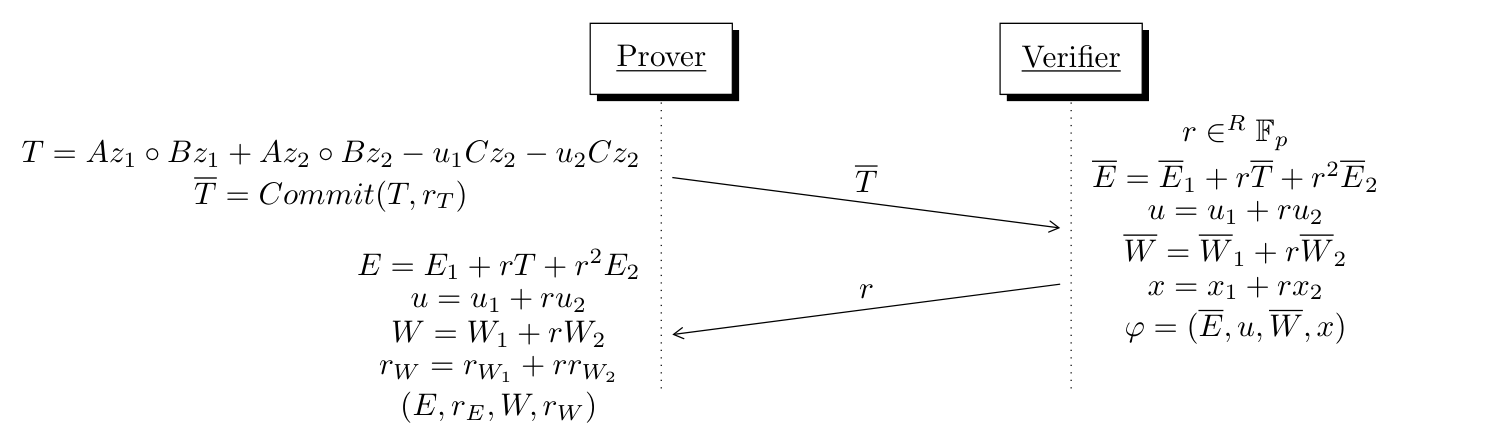
\includegraphics[width=\textwidth]{./imgs/interactive-FS-nova-diagram}

  Relation check:
  \begin{align*}
    &z=(1,x,W)\\
     &\begin{cases}
    Az \circ Bz - uCz - E \stackrel{?}{=} 0\\
    \overline{W} \stackrel{?}{=} Com(W)\\
    \overline{E} \stackrel{?}{=} Com(E)
  \end{cases}
  \end{align*}
\end{frame}

\begin{frame}{HyperNova NIMFS}
  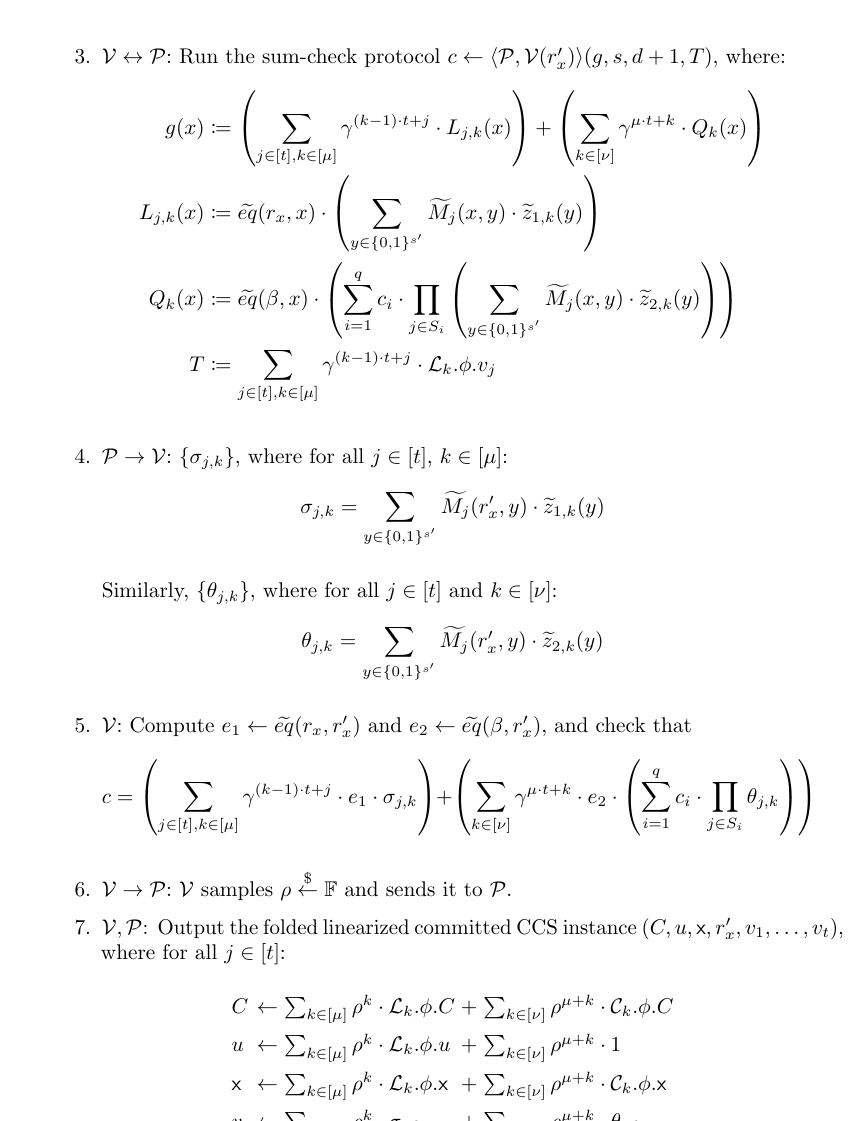
\includegraphics[width=8cm]{./imgs/hypernova-screenshot}
\end{frame}

\begin{frame}{ProtoGalaxy Folding}
  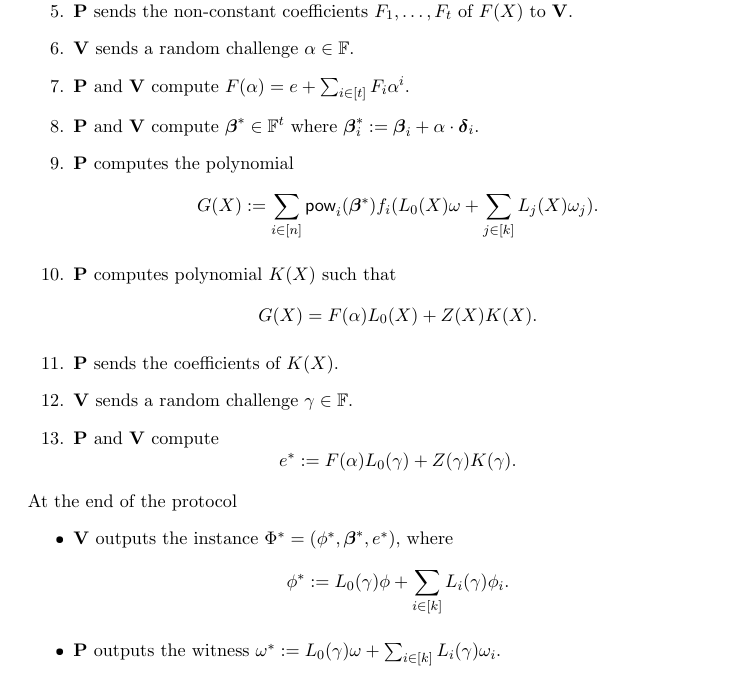
\includegraphics[width=8cm]{./imgs/protogalaxy-screenshot}
\end{frame}

\section[IVC]{IVC}

\begin{frame}{IVC}
  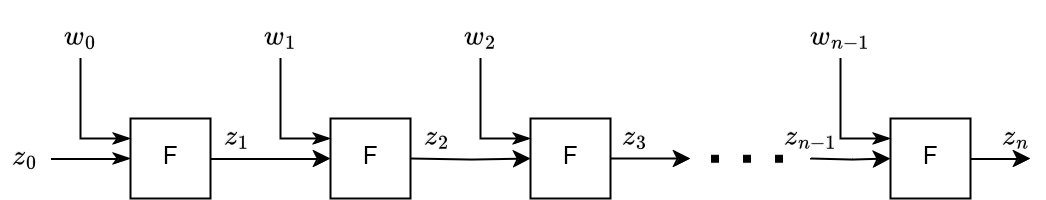
\includegraphics[width=\textwidth]{folding-main-idea-diagram}
  \begin{itemize}
    \item We have our folding protocol, in which P \& V 'fold' the instances (witness \& commitments)
    \item Will use it in the IVC setting
    \item at each IVC step, need to ensure that the 'folding' of the previous step was done correctly
    \item we 'augment' the circuit with extra checks that compute the folding Verifier
  \end{itemize}
\end{frame}

\begin{frame}{IVC - Nova example}
  \small{
  $U_i$ (\emph{running instance}): committed instance for the correct execution of invocations $1, \ldots, i-1$ of $F'$\\
  $u_i$ (\emph{incoming instance}): committed instance for the correct execution of invocation $i$ of $F'$
  }

  % draw: sketch of the Augmented F Circuit
  % big box for F', inside small box for F. NIFS.V box, how things connect to next iteration

  \vspace{4cm}
  
  \small{
  F':\\
  i) execute a step of the incremental computation, $z_{i+1} = F(z_i)$\\
  ii) invoke the NIFS.V to fold $U_i, u_i$ into $U_{i+1}$\\
  iii) other checks to ensure that the IVC is done properly
  }
\end{frame}

\begin{frame}{Cycle of curves}
  \small{
    NIFS.V involves $\mathbb{G}$ point operation, which are not native over $\mathbb{F}_r$ of $\mathbb{G}$.
  \\$\longrightarrow$ delegate them into a circuit over a 2nd curve 
  We use:
  \begin{itemize}
    \item $\mathbb{G}_1.\mathbb{F}_r = \mathbb{G}_2.\mathbb{F}_q$
    \item $\mathbb{G}_1.\mathbb{F}_q = \mathbb{G}_2.\mathbb{F}_r$
    \item eg. for Ethereum compatibility:\\
      $\mathbb{G}_1$: BN254, $\mathbb{G}_2$: Grumpkin.
  \end{itemize}

  \vspace{0.3cm}

  We 'mirror' the main $F'$ circuit into the 2nd curve\\
  each circuit computes natively the point operations of the other curve
  }

  % DRAW:
  % 1st the Nova with duplicated F' circuits over 2 curves
  % 2nd the Nova with CycleFold circuits sketch
\end{frame}


\begin{frame}{Augmented F Circuit + CycleFold Circuit}
  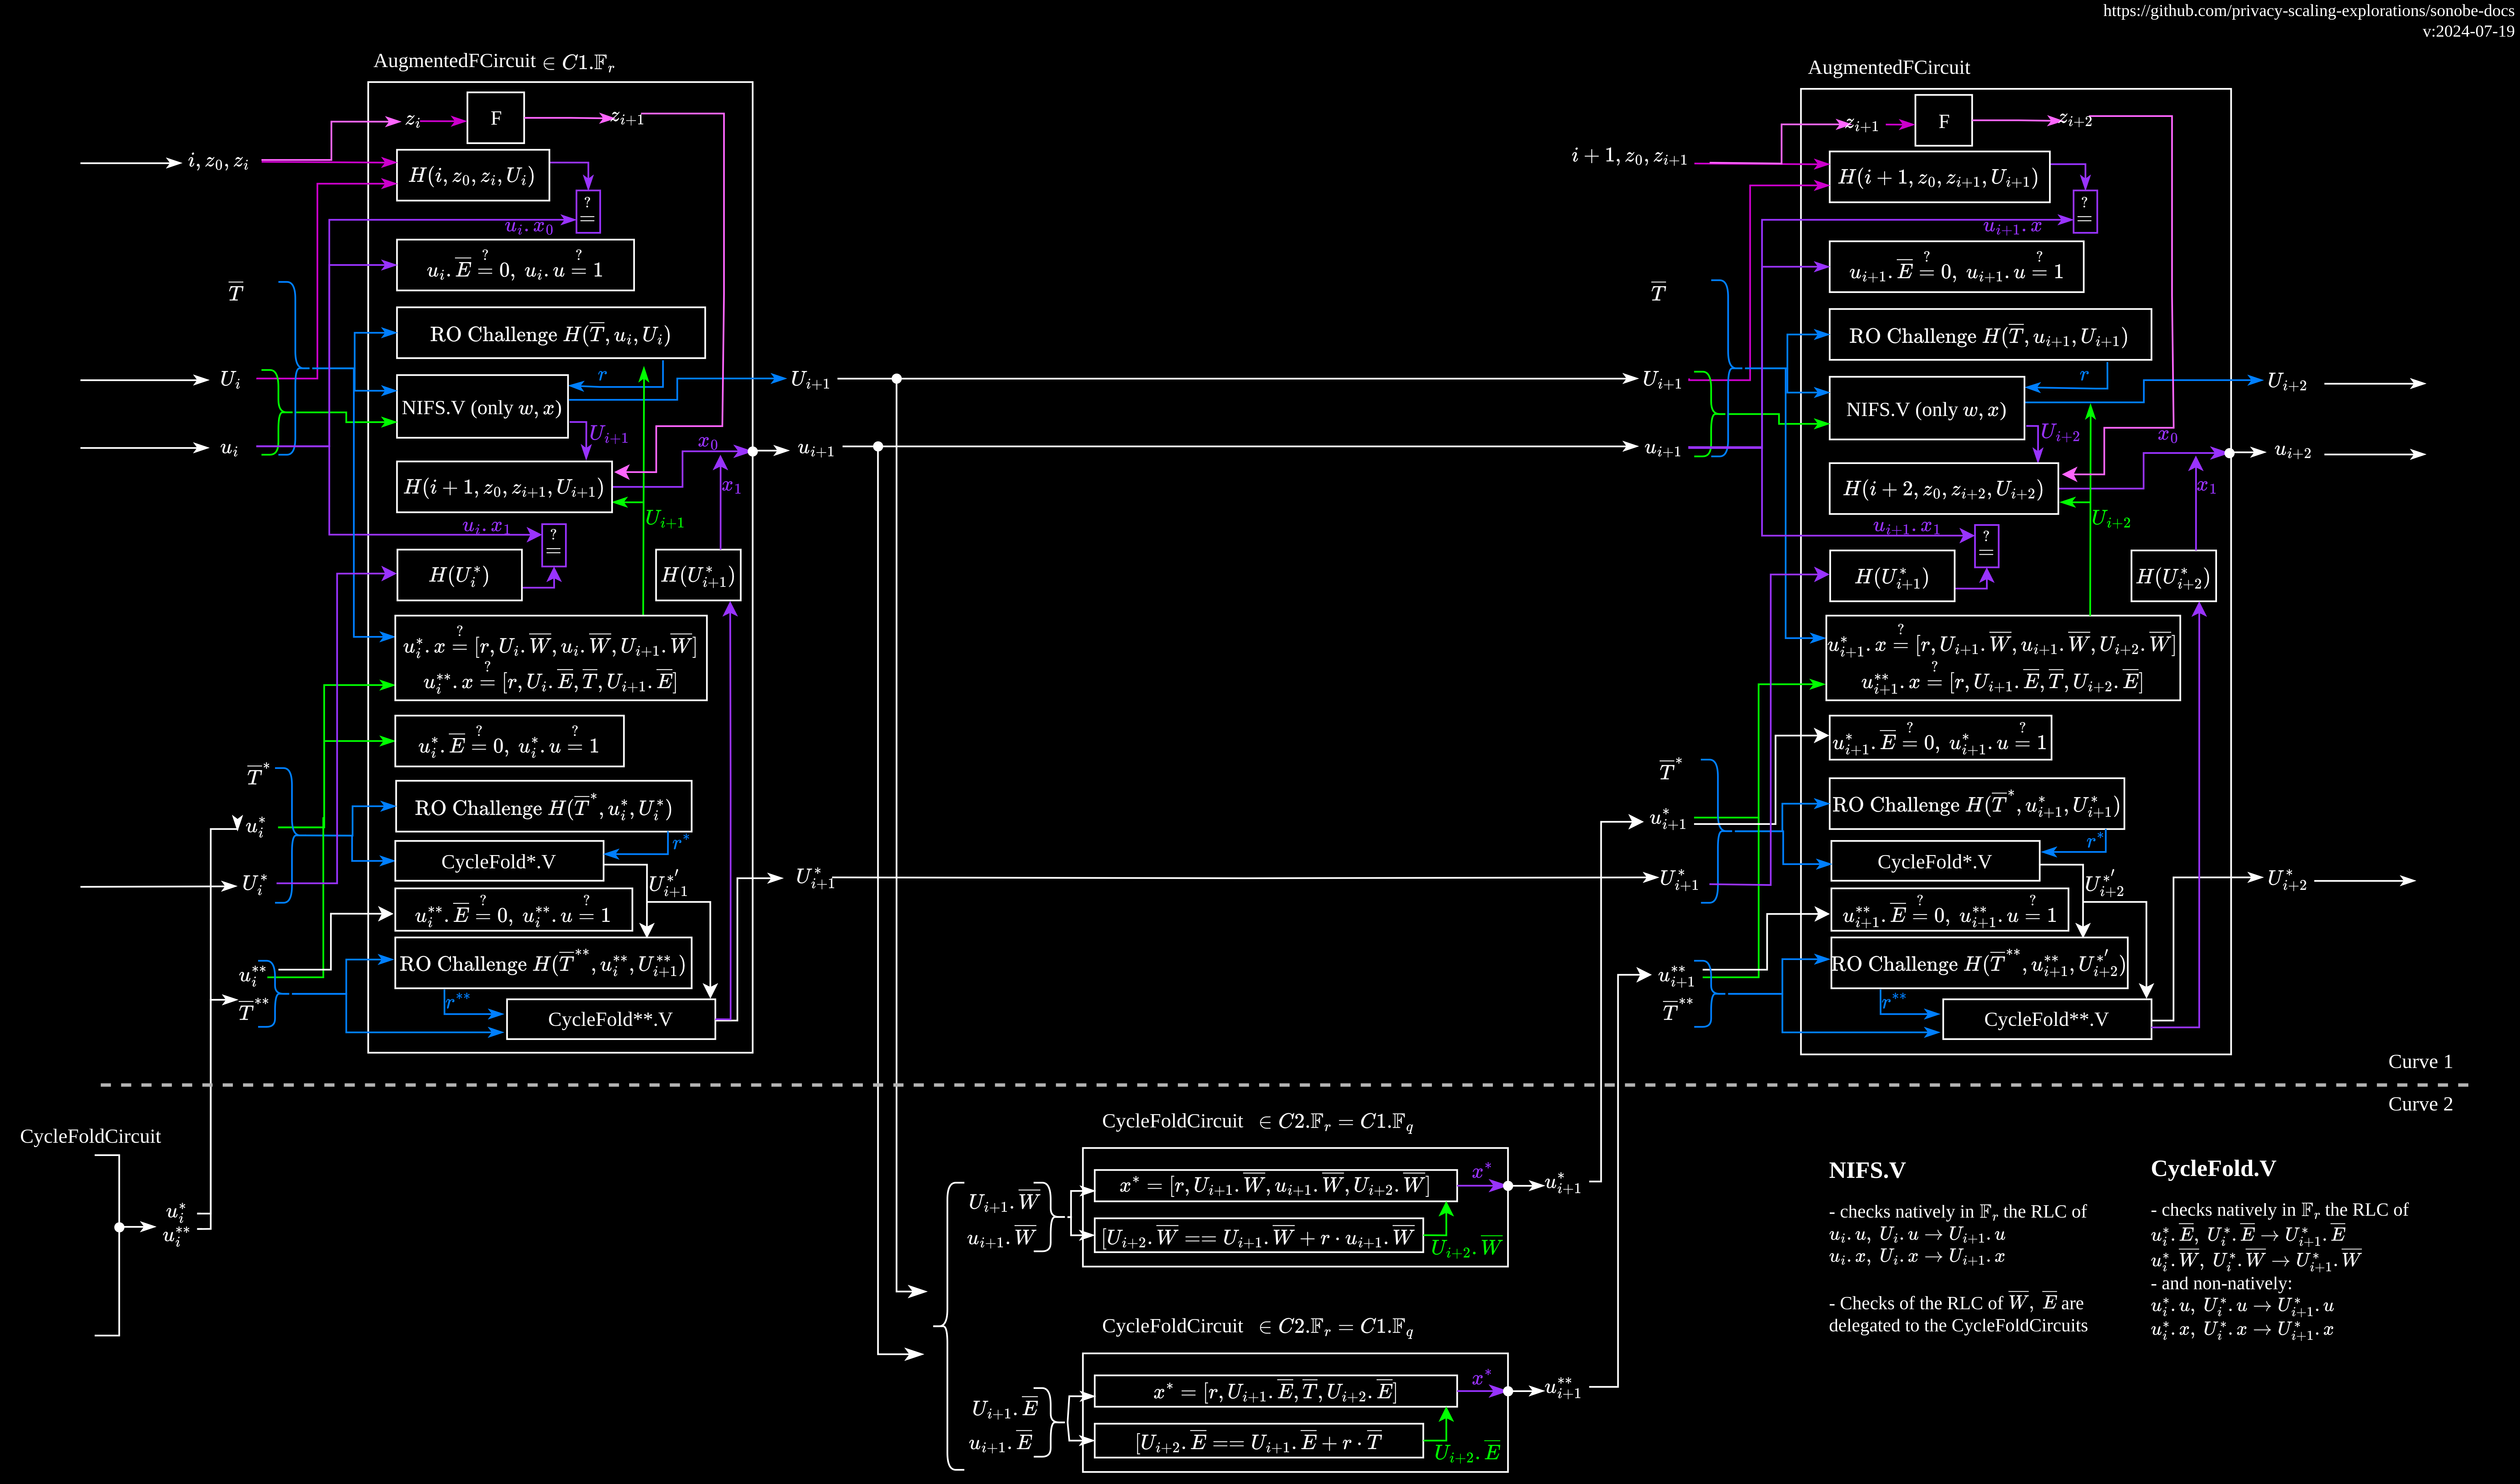
\includegraphics[width=\textwidth]{cyclefold-nova-diagram}
  % mention TODO folding overhead - num constraints of overhead, so for small circuits it is not worth
  explain: circuit overhead
\end{frame}

\begin{frame}{Adding zk to the IVC}
  \begin{itemize}
    \item fold the original witness with a randomized instance
    \item then we can delegate the rest of the computation to a third party server
  \end{itemize}
\end{frame}

\section{Decider (Final compressed proof)}

\begin{frame}{Decider (Final compressed proof)}
  \includegraphics[width=\textwidth]{cyclefold-paper-diagram}

  With Prover knowing the respective witnesses for $U_n, u_n, U_{EC,n}$

  \vspace{1cm}

  Issue: IVC proof is not succinct
\end{frame}

\begin{frame}{Decider}
  Original Nova: generate a zkSNARK proof with Spartan for $U_n, u_n, U_{EC, n}$\\
  $\longrightarrow$ 2 Spartan proofs, one on each curve\\
  (not EVM-friendly)

  % DRAW of the 2 circuits over the curves, and how we generate a Spartan proof for each one

\end{frame}

\begin{frame}{Decider}
  checks (simplified)
  \begin{enumerate}
    \item $(U_{n+1}, W_{n+1})$ satisfy Relaxed R1CS relation of AugmentedFCircuit
    \item verify commitments of $U_{n+1}.\{\overline{E}, \overline{W}\}$ w.r.t. $W_{n+1}.\{E,W\}$
    \item $(U_{EC,n}, W_{EC,n})$ satisfy Relaxed R1CS relation of CycleFoldCircuit
    \item verify commitments of $U_{EC,n}.\{\overline{E}, \overline{W}\}$ w.r.t. $W_{EC,n}.\{E,W\}$
    \item $u_n.E==0,~ u_n.u==1$, ie. $u_n$ is a fresh not-relaxed instance
    \item $u_n.x_0==H(n, z_0, z_n, U_n)$\\
          $u_n.x_1==H(U_{EC,n})$
    \item $NIFS.V(U_n, u_n)==U_{n+1}$
  \end{enumerate}

  % DRAW; by draw show which are native and not native
  % and that the NIFS.V we do it in Solidity
\end{frame}

\begin{frame}{Decider}
  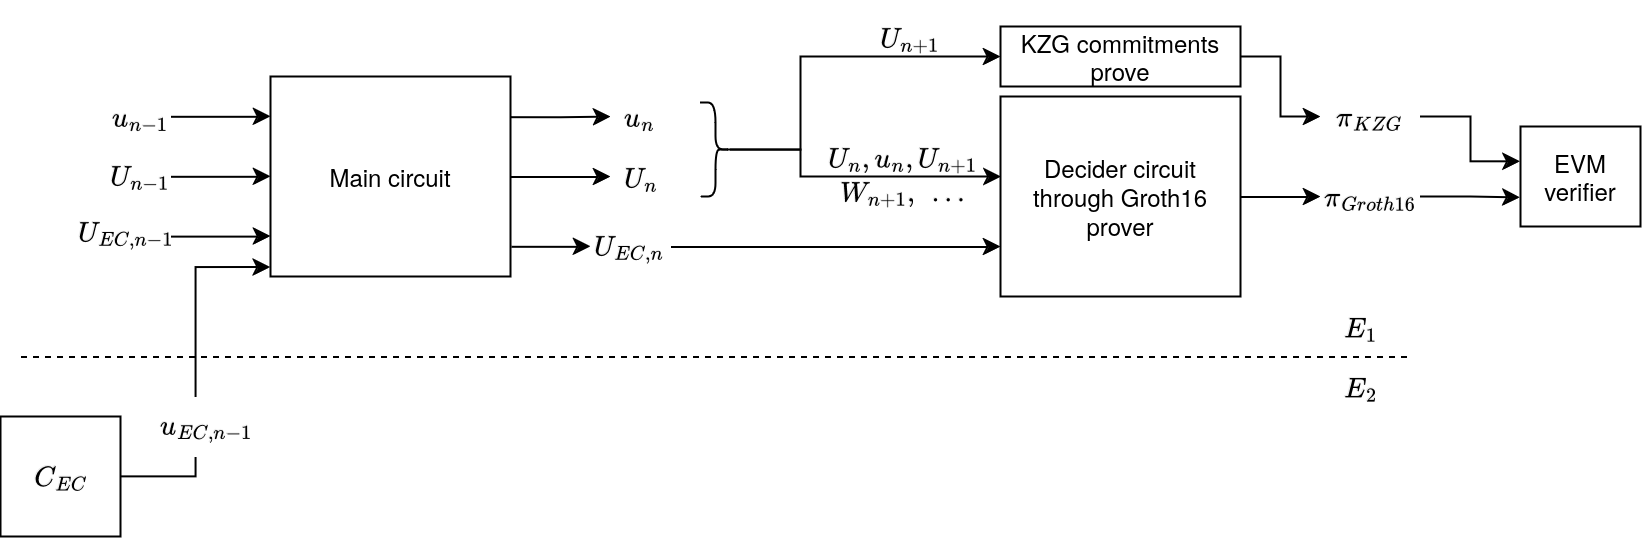
\includegraphics[width=\textwidth]{decider-onchain-flow-diagram}
  % DRAW of the full flow: from inputting the circuit, to folding to generating the Decider proof to verifying in Ethereum
\end{frame}

\section{Sonobe}
\begin{frame}{Sonobe}

  \footnotesize{
  Experimental folding schemes library implemented jointly by 0xPARC and PSE.\\
  \href{https://github.com/privacy-scaling-explorations/sonobe}{https://github.com/privacy-scaling-explorations/sonobe}
  \\Modular library,
  \begin{itemize}
    \item Be able to
    \begin{itemize}
      \item Add and test new folding schemes
      \item Compare schemes 'apples-to-apples'
      \item Researchers can easily add their own schemes (eg. Mova paper)
    \end{itemize}
    \item Make it easy for devs to use folding
    \begin{itemize}
      \item minimal code to fold your circuits ('plug-and-fold')
      \item easy to switch between folding schemes and curves
      \item support of multiple zk-circuit languages
    \end{itemize}
  \end{itemize}
  }
\end{frame}

\begin{frame}{Sonobe - Dev experience}
  \footnotesize{

  Dev flow:
  \begin{enumerate}
    \item Define a circuit to be folded
    \item Set which folding scheme to be used (eg. Nova with CycleFold)
    \item Set a final decider to generate the final proof (eg. Groth16 over BN254 curve)
    \item Generate the the decider verifier (EVM Solidity contract)
  \end{enumerate}
  }

  \vspace{1cm}

  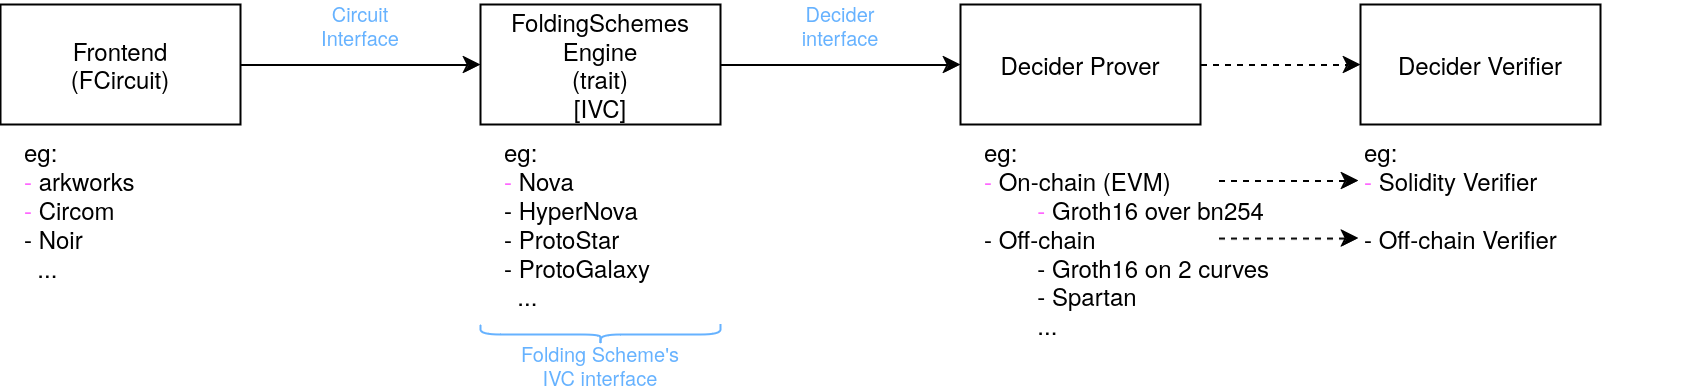
\includegraphics[width=\textwidth]{sonobe-lib-pipeline}
\end{frame}


\begin{frame}{Status of Sonobe - dev experience}
  \begin{itemize}
    \item Verify in Ethereum
    \begin{itemize}
      \item solidity verifier contract generator
    \end{itemize}
    \item Frontends - how can the dev define a circuit to be folded
    \begin{itemize}
      \item Arkworks \href{https://github.com/arkworks-rs/}{https://github.com/arkworks-rs/}
      \item Circom \href{https://github.com/iden3/circom}{https://github.com/iden3/circom}
      \item Noir \href{https://noir-lang.org/}{https://noir-lang.org/}
      \item Noname \href{https://github.com/zksecurity/noname}{https://github.com/zksecurity/noname}
    \end{itemize}
  \end{itemize}
\end{frame}

\begin{frame}{Status of Sonobe - schemes implemented}
  \scriptsize{

  Implemented:
  \begin{itemize}
    \item \textbf{Nova}: Recursive Zero-Knowledge Arguments from Folding Schemes\\ \href{https://eprint.iacr.org/2021/370.pdf}{https://eprint.iacr.org/2021/370.pdf}, Abhiram Kothapalli, Srinath Setty, Ioanna Tzialla. 2021
    \item \textbf{CycleFold}: Folding-scheme-based recursive arguments over a cycle of elliptic curves\\ \href{https://eprint.iacr.org/2023/1192.pdf}{https://eprint.iacr.org/2023/1192.pdf}, Abhiram Kothapalli, Srinath Setty. 2023
    \item \textbf{HyperNova}: Recursive arguments for customizable constraint systems\\ \href{https://eprint.iacr.org/2023/573.pdf}{https://eprint.iacr.org/2023/573.pdf}, Abhiram Kothapalli, Srinath Setty. 2023
  \end{itemize}
  Almost finished:
  \begin{itemize}
    \item \textbf{ProtoGalaxy}: Efficient ProtoStar-style folding of multiple instances\\ \href{https://eprint.iacr.org/2023/1106.pdf}{https://eprint.iacr.org/2023/1106.pdf}, Liam Eagen, Ariel Gabizon. 2023
  \end{itemize}
  Soon:
  \begin{itemize}
    \item \textbf{Mova}: Nova folding without committing to error terms\\ \href{https://eprint.iacr.org/2024/1220.pdf}{https://eprint.iacr.org/2024/1220.pdf}, Nikolaos Dimitriou, Albert Garreta, Ignacio Manzur, Ilia Vlasov. 2024
  \end{itemize}
  Temptative:
  \begin{itemize}
    \item \textbf{LatticeFold}: A Lattice-based Folding Scheme and its Applications to Succinct Proof Systems\\ \href{https://eprint.iacr.org/2024/257.pdf}{https://eprint.iacr.org/2024/257.pdf}, Dan Boneh, Binyi Chen. 2024
    \item Parallel folding
  \end{itemize}

  }
\end{frame}

\begin{frame}{Code example}
  [show code with a live demo]
\end{frame}

\begin{frame}{Code example}
  \footnotesize{
  Some numbers (still optimizations pending):
  \begin{itemize}
  \item AugmentedFCircuit (Nova): $\sim 50k$ R1CS constraints
  \item DeciderEthCircuit: $\sim 10M$ R1CS constraints
  \begin{itemize}
    \item $<3$ minutes in a 32GB RAM 16 core laptop
  \end{itemize}
  \item gas costs (DeciderEthCircuit proof): $\sim 800k$ gas
  \begin{itemize}
    \item mostly from G16, KZG10, public inputs processing
    \item will be reduced by hashing the public inputs
    \item expect to get it down to $< 500k$ gas.
  \end{itemize}
  \end{itemize}
  }

  \vspace{0.6cm}

  Recall, this proof is proving that applying $n$ times the function $F$ (the circuit that we're folding) to an initial state $z_0$ results in the state $z_n$.

  \vspace{0.4cm}

  In Srinath Setty words, you can prove practically unbounded computation onchain by 800k gas (and soon $< 500k$).
\end{frame}

\begin{frame}{Wrappup}
\begin{itemize}
  \item \href{https://github.com/privacy-scaling-explorations/sonobe}{https://github.com/privacy-scaling-explorations/sonobe}
  \item \href{https://privacy-scaling-explorations.github.io/sonobe-docs/}{https://privacy-scaling-explorations.github.io/sonobe-docs/}
\end{itemize}

  \begin{center}
    
\includegraphics[width=5cm]{./imgs/sonobe-link-qrcode}
  \end{center}

\tiny{
  $$\text{2024-08-08}$$
  $$\text{\href{https://0xparc.org}{0xPARC}~\&~\href{https://pse.dev/}{PSE.}}$$
}
\end{frame}

\end{document}
